\section{Overview} % (fold)
\label{sec:overview}
    
    Per il seguente progetto si è scelto di analizzare il famoso puzzle/problema di ottimizzazione chiamato \emph{Eternity 2}, attraverso euristiche basate su ricerca locale.

    Anche alla luce di quanto studiato, sono state selezionate le seguenti mosse e i relativi intorni:

    \paragraph{\emph{Even Chessboard} e \emph{Odd Chessboard Move}} % (fold)
    \label{par:even_odd}
        La mossa prevede la selezione di tile alternate della \emph{board} di gioco (si immagini in questo senso di avere una scacchiera e di selezionare solamente le pedine in posizioni nere, o alternativamente, bianche). Si noti che le pedine non selezionate sono sufficienti a poter calcolare in modo semplice ed agevole il $\Delta$--costo di una data mossa.

        \begin{figure}[H]
            \centering
            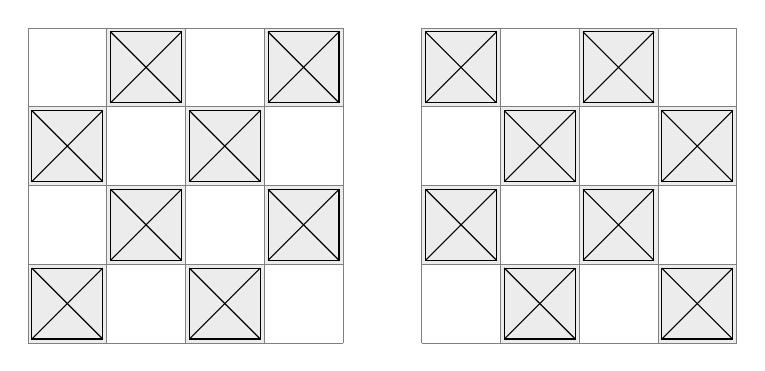
\begin{tikzpicture}
                \foreach \x/\y in {0/0,0/2,1/1,1/3,2/0,2/2,3/1,3/3,5/1,5/3,6/0,6/2,7/1,7/3,8/0,8/2}
                {
                    \fill[fill=gray!15!white] (\x,\y) rectangle (\x+1,\y+1);
                    \draw[black] (\x+.05,\y+.05) rectangle (\x+.95,\y+.95);
                    \draw[black] (\x+.05,\y+.05) -- (\x+.95,\y+.95);
                    \draw[black] (\x+.95,\y+.05) -- (\x+.05,\y+.95);
                }
                \draw[step=1cm,gray,very thin] (0,0) grid (4,4);
                \draw[step=1cm,gray,very thin] (5,0) grid (9,4);
            \end{tikzpicture}
            \caption{Even and Odd tile selection}
        \end{figure}

    % paragraph even_odd (end)

    \paragraph{Singleton Move} % (fold)
    \label{par:singleton}
    
    % paragraph singleton (end)

    \paragraph{L Move} % (fold)
    \label{par:l}
    
    % paragraph l (end)

    \paragraph{Three--Tile Move} % (fold)
    \label{par:three_tile_move}
    
    % paragraph three_tile_move (end)

%    Componenti delle mosse e componenti dello stato. Come abbiamo diviso la selezione dal ricombinamento.
%
%    Mosse scelte
%
%    implementazione della SelectBest con Hungarian algorithm, esplorazione polinomiale di un intorno esponenziale 
%
%    tecniche scelte
%    simulated anealing con mossa 3-modale (singleton, even, odd)
%    simulated anealing con mosse 3-modali (singleton, tts, L)
%
%    steepest descend (singleton)
%    steepest descend (tts)
%    steepest descend (L)
%
%    perchè non sono state usate mosse multimodali per steepest descend.


    
% section overview (end)